\section{Versuchsbeschreibung}

\subsection{Versuchsaufbau}
\begin{figure}[H]
\centering 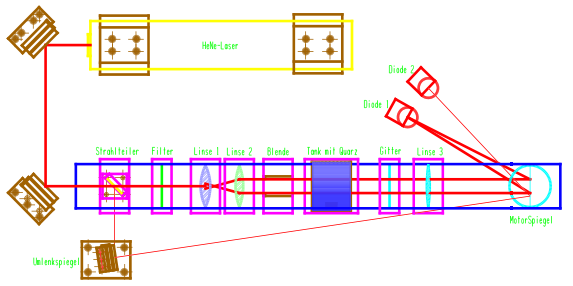
\includegraphics[width = \textwidth]{Bilder/Aufbau.jpg}
\caption{Schematischer Versuchsaufbau}
\end{figure}



\subsection{Durchf\"uhrung}

Mit einem He-Ne Laser, der monochromatisches Licht der Wellenl\"nge $\lambda = 6328 \mathring{A}$ abstrahlt, untersuchen wir das Beugungsph\"anomen an verschiedenen Gittern und bestimmen daraus die Gitterkonstanten bzw. Aperturfunktionen dieser Gitter. Bei einem Ultraschallgitter versuchen wir au\ss erdem die Schallwellenl\"ange in einer Isooktan-L\"osung herauszufinden und vergleichen unsere Messergebnisse mit der Raman-Nath-Theorie.

\subsubsection{Sinusgitter}

Wir richten den Laserstrahl senkrecht auf das Sinusgitter ohne Aufweitung und ohne Kollimationslinse, da bei diesem Gitter die 0. und die 1. Ordnung problemlos unterscheidbar sind. Auf einem Schirm hinter dem Gitter kann man das Beugungsmuster direkt beobachten und somit die Gitterkonstante bestimmen.

\subsubsection{Amplitudengitter}

Die H\"ohen der Linsen werden korrekt justiert und der Strahl wird durch Verschiebung der Blende auf Parallelit\"at \"uberpr\"uft. Wir bauen dann den Strahlteiler ein und nacheinander die Linsen. Diese werden mit der Blende justiert, damit der Strahlengang parallel bleibt. Die 3. Linse wird auf den Drehspiegel justiert. Die Dioden werden so eingestellt, dass sie die maximale Signalintensit\"at aufnehmen k\"onnen. Der Oszillator wird so eingestellt, dass das Bild m\"oglichst stabil ist. Schlussendlich eichen wir die Zeitachse des Oszilloskopenbildes anhand des Gitters "R". Anhand der Distanzen (Zeiten) zwischen dem Hauptmaximum und aller sichtbaren Beugungsordnungen auf dem Oszilloskop f\"ur alle Gitter, bestimmen wir durch lineare Regression die Umrechnungformel von Zeiten in Brechungswinkel.
Mit dem so justierten Aufbau bestimmen wir jetzt die Gitterkonstanten von fünf Gittern.

\subsubsection{Aperturfunktion}
Für das Gitter mit der größten Gitterkonstanten bestimmen wir die Intensitäten der sichtbaren Maxima und berechnen wie in 2.1.2. beschrieben die Aperturfunktion anhand der Fourierreihe. Wir zeichnen dann eine Periode dieser Funktion.

\subsubsection{Verh\"altnis von Spaltbreite zu Spaltabstand}

Um die Spaltbreite zu erhalten, messen wir die Halbwertsbreite der Maxima der berechneten Aperturfunktion. Der Spaltabstand ergibt sich aus der Differenz einer Periode und der Spaltbreite. Wir berechnen dann das Verh\"altnis dieser beiden Gr\"o\ss en.

\subsubsection{Aufl\"osungsverm\"ogen der Gitter}

Wir messen die Breite des Laserstrahls und ermitteln mit der berechneten Gitterkonstanten die Anzahl der durchleuchteten Gitterst\"abe. Hieraus und aus der Anzahl der sichtbaren Maxima k\"onnen wir die Aufl\"osung der Gitter berechnen.



\subsubsection{Raman-Nath-Theorie}

An Stelle des Gitters setzten wir die Ultraschallzelle ein. Der Laser wird beim Durchgang durch die Ultraschallzelle gebeugt und wir nehmen mittels des Drehspiegels und der Dioden die Intensitätsverteilung der Beugungsfigur auf. Da die Verteilung von der Amplitude der Dichteschwankungen abhängt und diese Proportional zum Quadrat der angelegten Spannung ist, nehmen wir eine Messreihe für verschiedene Spannungen auf. Diese vergleichen wir dann mit der Raman-Nath-Theorie (siehe 2.2) und können durch Vergleich mit dem theoretischen Wert außerdem die Schallwellenlänge bestimmen.

\clearpage










